% !TEX program = xelatex
% !BIB program = biber
% =====================================================================
%  Beamer template — adapted from weibo-hot/paper/pre/journal.club
%  Compile with XeLaTeX + Biber:  latexmk -xelatex main.tex
% =====================================================================
% \documentclass[draft]{beamer}
\documentclass[]{beamer}
\usetheme{Berlin}
\usepackage{hyperref}
\hypersetup{colorlinks=true,urlcolor=blue,linkcolor=.,citecolor=.,filecolor=.}
\usepackage{graphicx}   % figures
\graphicspath{{../figures/}}
\usepackage{multicol}   % multi-column layouts
\usepackage{booktabs}   % tables
\usepackage{subfigure}  % sub-figures
\usepackage{xcolor}
\usepackage{color}
\usepackage{csquotes}
\usepackage{xltxtra}
\usepackage{xelatexemoji}
\usepackage[style=apa,sortcites=true,sorting=nyt,backend=biber]{biblatex}
\addbibresource{refs.bib}
\usepackage{tikz}       % DAG graphs
\usetikzlibrary{shapes,decorations,arrows,calc,arrows.meta,fit,positioning}

\setbeamertemplate{caption}{\raggedright\insertcaption\par}
\setbeamerfont{caption}{size=\tiny}   % captions: tiny + gray
\setbeamercolor{caption}{fg=gray}
\setbeamertemplate{footline}{}
\tikzset{
  -Latex,auto,node distance =1 cm and 1 cm,semithick,
  state/.style ={ellipse, draw, minimum width = 0.7 cm},
  block/.style ={rectangle, draw, minimum width = 0.7 cm},
  point/.style = {circle, draw, inner sep=0.04cm,fill,node contents={}},
  bidirected/.style={Latex-Latex},
  el/.style = {inner sep=2pt, align=left, sloped}
}

% ---------- Colours ----------
\definecolor{green}{RGB}{62, 138, 46}
\definecolor{blue}{RGB}{3, 105, 170}
\definecolor{red}{RGB}{194, 54, 55}

\usecolortheme{beaver}

\definecolor{primary}{RGB}{0,24,49}
\definecolor{secondary}{RGB}{0,48,96}
\definecolor{tertiary}{RGB}{94,48,0}
\definecolor{quaternary}{RGB}{94,48,0}
\setbeamercolor{titlelike}{parent=palette secondary,fg=white}
\setbeamercolor{frametitle}{bg=primary!60!white}
\setbeamercolor{frametitle right}{bg=primary!60!white}
\setbeamercolor*{palette primary}{bg=primary, fg = white}
\setbeamercolor*{palette secondary}{bg=secondary, fg = white}
\setbeamercolor*{palette tertiary}{bg=tertiary, fg = white}
\setbeamercolor*{palette quaternary}{bg=quaternary, fg = white}

\definecolor{nus_blue}{rgb}{0,0.24,0.49}
\definecolor{nus_yellow}{rgb}{0.94, 0.48, 0.00}
\definecolor{nus_yellow_highlight}{rgb}{0.94, 0.48, 0.00}

\setbeamercolor{section in toc}{fg=black,bg=white}
\setbeamercolor{alerted text}{fg=nus_blue!80!gray}
\setbeamercolor{navigation symbols}{fg=gray!60!black, bg=gray!10!white}
\setbeamercolor{navigation symbols dimmed}{fg=gray!50!black}
\setbeamercolor*{palette primary}{fg=black!60!black,bg=gray!15!white}
\setbeamercolor*{palette secondary}{fg=black!70!black,bg=gray!15!white}
\setbeamercolor*{palette tertiary}{bg=black!80!black,fg=gray!10!white}
\setbeamercolor*{palette quaternary}{fg=black,bg=gray!5!white}
\setbeamercolor{enumerate item}{fg=black,bg=white}
\setbeamercolor{itemize item}{fg=black,bg=white}
\setbeamercolor{item}{fg=black,bg=white}
\setbeamercolor*{sidebar}{fg=black,bg=gray!15!white}

\setbeamercolor*{palette sidebar primary}{fg=black!10!black}
\setbeamercolor*{palette sidebar secondary}{fg=white}
\setbeamercolor*{palette sidebar tertiary}{fg=black!50!black}
\setbeamercolor*{palette sidebar quaternary}{fg=gray!10!white}

\setbeamercolor{button}{bg=white,fg=black}
\setbeamercolor{author in head/foot}{bg=black}
\setbeamercolor{title in head/foot}{bg=black!20}
\setbeamercolor{titlelike}{bg=black!100!white}
\setbeamercolor{frametitle}{bg=black!100!white}
\setbeamercolor{frametitle right}{bg=black!100!white}
\setbeamercolor{empty}{bg=black}

% ---------- Headline (section navigation) & frame title ----------
\setbeamertemplate{headline}{%
  \begin{beamercolorbox}[wd=\paperwidth,ht=3.5ex,dp=3.5ex]{section in head/foot}
    \insertnavigation{\paperwidth}%
  \end{beamercolorbox}%
}

\setbeamertemplate{frametitle}{%
  \nointerlineskip%
  \begin{beamercolorbox}[wd=\paperwidth,leftskip=.3cm,rightskip=.3cm plus1fil,vmode]{frametitle}
    \vskip0.5ex%
    \usebeamerfont*{frametitle}\strut\insertframetitle\strut\par%
    \vskip0.05ex%
  \end{beamercolorbox}%
}

\setbeamercolor*{separation line}{}
\setbeamercolor*{fine separation line}{}
\setbeamercolor{bibliography entry author}{fg=black}
\setbeamercolor{bibliography entry title}{fg=black}
\setbeamercolor{bibliography entry location}{fg=black}
\setbeamercolor{bibliography entry note}{fg=black}
\setbeamertemplate{bibliography item}{}

% ---------- CJK support ----------
\usepackage{xeCJK}

% ---------- Helper macros ----------
\providecommand{\tabfnm}[1]{\textsuperscript{#1}}  % apa7 marker used by \input tables
\newcommand{\hlt}[1]{\textcolor{red}{\textbf{#1}}}
% Citation styling: footnotes and \parencite are gray + tiny everywhere;
% \textcite keeps the surrounding text style (black, normal size in body text).
\setbeamerfont{footnote}{size=\tiny}
\setbeamercolor{footnote}{fg=gray}
\setbeamercolor{footnote mark}{fg=gray}
\newcommand{\mkgrayparens}[1]{{\tiny\color{gray}\mkbibparens{#1}}}
\DeclareCiteCommand{\parencite}[\mkgrayparens]
  {\usebibmacro{cite:init}\usebibmacro{prenote}\toggletrue{apa:inpcite}}
  {\usebibmacro{citeindex}\usebibmacro{cite}\usebibmacro{cite:post}}
  {}
  {\usebibmacro{postnote}\togglefalse{apa:inpcite}}
\DeclareMultiCiteCommand{\parencites}[\mkgrayparens]{\parencite}{\setunit{\multicitedelim}}
\newcommand{\citegray}[1]{\parencite{#1}}  % legacy alias
\newcommand{\sourcenote}[1]{{\let\thefootnote\relax\footnotetext{#1}}}  % unnumbered gray/tiny footnote
\newcommand{\referencesize}{\tiny}
\renewcommand*{\bibfont}{\referencesize}

% Black divider slide. \sectionframe{Title} also starts a \section, so the
% headline navigation highlights correctly. Use \dividerframe{Title} for a
% divider without a new section (e.g. Acknowledgments, References).
\newcommand{\dividerframe}[1]{%
  {\setbeamercolor{background canvas}{bg=black}%
   \begin{frame}
     \begin{center}\Huge{\textcolor{white}{#1}}\end{center}
   \end{frame}}%
}
\newcommand{\sectionframe}[1]{\section{#1}\dividerframe{#1}}

% ---------- Title page ----------
\title[AI in Quantitative Social Research]{Responsibly deploy AI in Quantitative Social Research}
\author[Rongxin Ouyang]{Rongxin Ouyang$^{*}$}
\institute{\textcolor{gray}{
    $^{*}$ PhD Candidate in Computational Communication, National University of Singapore; rongxin@u.nus.edu\\
Research Interest: Using causal and computational methods to evaluate societal and political impacts of digital information technologies}}
\date{\small \textcolor{gray}{November 5, 2026}}

\begin{document}

\frame{\titlepage}

\begin{frame}
  \frametitle{The goal of this session}
  \begin{columns}[T,onlytextwidth]
    \column{0.48\textwidth}
        \large \textcolor{gray}{... lower barrier (of computational skills) ... redistribution of  expertise ... } ``For students, the question is no longer whether they can \textcolor{orange}{code}, but whether they can \textcolor{blue}{audit, critique, adapt, and responsibly deploy} AI-assisted methods without mistaking convenience''
    \column{0.5\textwidth}
      \begin{figure}
        \centering
        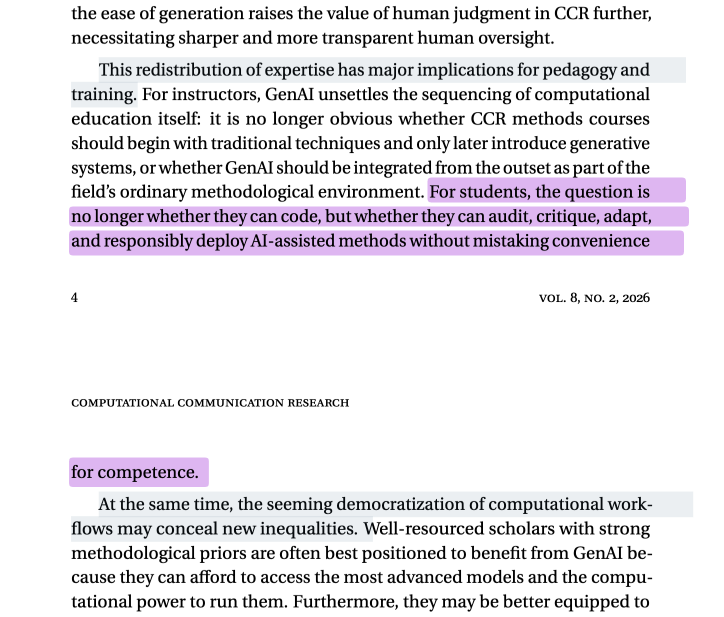
\includegraphics[width=\linewidth]{responsively.use.png}
        \caption{Source: \textcite{zhou2026be} (pp.~4--5)}
      \end{figure}
  \end{columns}
\end{frame}

% =====================================================================
\sectionframe{Introduction}
% =====================================================================

\begin{frame}
  \frametitle{What Is AI?}
  \begin{columns}[T,onlytextwidth]
    \column{0.55\textwidth}
      \begin{itemize}
        \item ``The science and engineering of making intelligent machines'' \textcolor{gray}{\tiny (McCarthy)}
        \item Systems that \hlt{perceive} their environment and \hlt{act} to achieve goals
        \item A nested family of techniques, not a single technology
      \end{itemize}
    \column{0.45\textwidth}
      \begin{center}
        \begin{tikzpicture}[-,every node/.style={font=\tiny}]
          \draw[fill=gray!10] (0,0) ellipse (2.2 and 1.6);
          \draw[fill=gray!25] (0,-0.3) ellipse (1.7 and 1.2);
          \draw[fill=gray!40] (0,-0.6) ellipse (1.2 and 0.8);
          \draw[fill=red!30]  (0,-0.85) ellipse (0.7 and 0.45);
          \node at (0,1.3)   {Artificial Intelligence};
          \node at (0,0.6)   {Machine Learning};
          \node at (0,-0.1)  {Deep Learning};
          \node at (0,-0.85) {LLMs};
        \end{tikzpicture}
      \end{center}
  \end{columns}
\end{frame}

\begin{frame}
  \frametitle{A Brief History of AI}
  \footnotesize
  \begin{itemize}
    \item Observation: Artificial intelligence is a general field developed decades ago (singple-poatrone); Early tools mainly classified, clustered, or predicted from human-produced traces \parencite{zhou2026be}.
    \item Roughly into pre-LLM and LLM eras for the goal of this session
  \begin{itemize}
    \item Before the introduction of Transformers \parencite{vaswani2017attention}, a model structure designed to parallelize training, we have traditional machine learning models such as logistic regression, SVMs, and early neural networks
    \item After the introduction of Transformers, large-scale pre-trained language models such as BERT and GPT series became prominent, enabling more general-purpose natural language understanding and generation tasks, such as generative language models and conversational agents
    \item Specifically, we focuse on the LLM era post-2020 \parencite[marked by GPT-3; ][]{xu2026large} and its implications for computational social science research
  \end{itemize}
  \end{itemize}
\end{frame}

% =====================================================================
\sectionframe{Pre-LLMs AI}
% =====================================================================

\begin{frame}
  \frametitle{The use of Pre-LLM AI in Quantitative Social Research}
  \begin{columns}[T,onlytextwidth]
    \column{0.5\textwidth}
      \setbeamerfont{itemize/enumerate body}{size=\footnotesize}
      \footnotesize
      \begin{itemize}
        \item \textbf{Supervised learning}: hand-label a sample, train a classifier, scale up
        \item \textbf{Unsupervised learning}: topic models, clustering, word embeddings
        \item \textbf{Text, images, and networks as data}~\citegray{king2013how}
        \item \textbf{ML for causal inference}: heterogeneous effects, high-dimensional controls
      \end{itemize}
      ~\\
      \textcolor{gray}{Common thread: task-specific models, labeled data, and a researcher-built pipeline}
    \column{0.48\textwidth}
      \begin{figure}
        \centering
        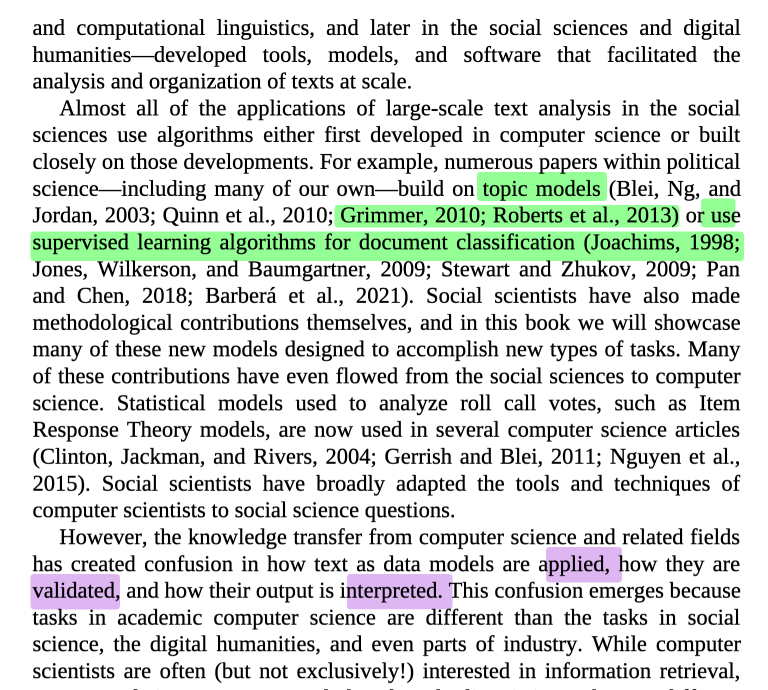
\includegraphics[width=\linewidth]{use.pre.llm.png}
        \caption{Source: \textcite{grimmer2022text} (p.23) }
      \end{figure}
  \end{columns}
\end{frame}

% =====================================================================
\sectionframe{LLMs}
% =====================================================================

\begin{frame}
  \frametitle{Roles of LLMs in Computational Social Science}
  \begin{center}
    \itemize{
      \item A recent review article suggests four roles of LLMs in computational social science: Subject, Assistant, Collaborator, Evaluator
    }
    \end{center}
    \begin{figure}
      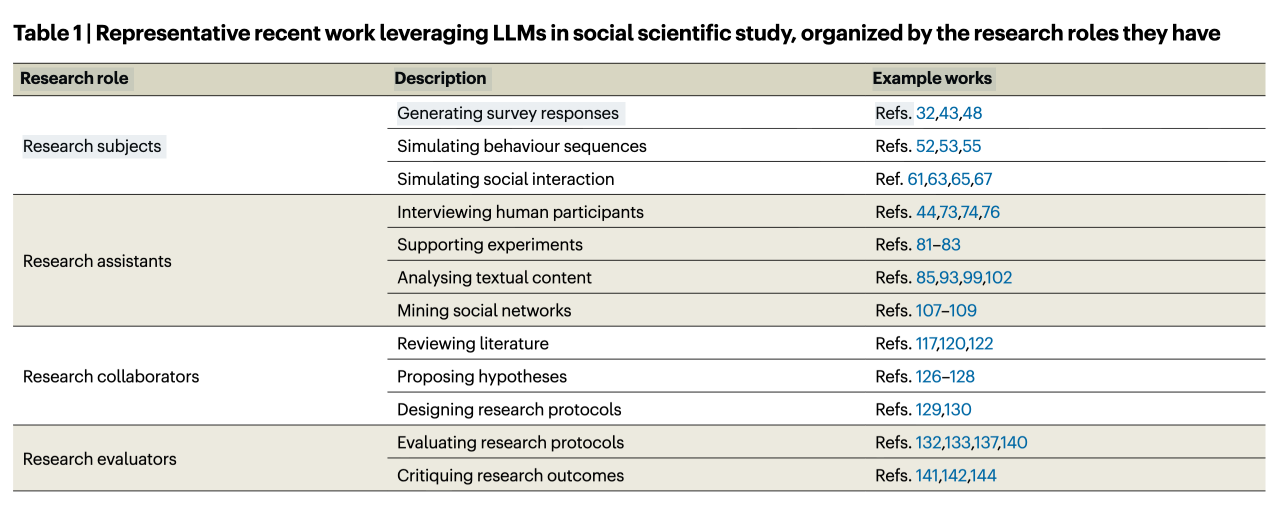
\includegraphics[width=\linewidth]{../figures/review.tab.1.png}
    \end{figure}
\end{frame}

\begin{frame}
  \frametitle{Roles of LLMs in Computational Social Science}
  \begin{center}
    \itemize{
      \item By adopting more recent perspectives, we may propose a more comprehensive categorization of LLM roles in CSS; to be elaborated in the following slides
    }
  \end{center}
  \begin{center}
    \begin{tikzpicture}[-Latex]
      \node[block, minimum width=2.4cm, minimum height=0.9cm] (s) at (0,0)   {\small \textbf{Subject}};
      \node[block, minimum width=2.4cm, minimum height=0.9cm] (m) at (4,0)   {\small \textbf{Method}};
      \node[block, minimum width=2.4cm, minimum height=0.9cm] (o) at (8,0)   {\small \textbf{Object}};
      \node[font=\tiny, align=center] at (0,-1) {LLM \emph{stands in}\\for humans};
      \node[font=\tiny, align=center] (ml) at (4,-1) {LLM \emph{does}\\research work};
      \node[font=\tiny, align=center] at (8,-1) {LLM \emph{is studied}};
      \node[state, font=\tiny] (a) at (1.9,-2.6) {Assistant};
      \node[state, font=\tiny] (c) at (4,-2.6)   {Collaborator};
      \node[state, font=\tiny] (e) at (6.1,-2.6) {Evaluator};
      \path (ml) edge (a) (ml) edge (c) (ml) edge (e);
    \end{tikzpicture}
  \end{center}
  \sourcenote{Source: Four roles (subjects, assistants, collaborators, evaluators) categorized in \textcite{xu2026large}; four categories thought from \textcite{liang2026computational}; and two roles (a research tool, an object of inquiry) adapted from \textcite{zhou2026be}}
\end{frame}


\begin{frame}
  \frametitle{AI as Subject: Categories}
      \footnotesize
      \begin{itemize}
        \item LLMs serve as research subjects
        \begin{itemize}
          \item Generate survey responses 
          \item Simulating behavior sequences
          \item Simulating social interactions
        \end{itemize}
      \end{itemize}
\end{frame}

\begin{frame}
  \frametitle{AI as Subject: Pros and Cons}
  \begin{columns}[T,onlytextwidth]
    \column{0.6\textwidth}
      \footnotesize
      \begin{itemize}
        \item \textbf{Pros:}
      \begin{itemize}
      \item Successfully replicate human responses \parencite{argyle2023out}
      \end{itemize}
    \end{itemize}
    \column{0.4\textwidth}
      \begin{figure}
        \centering
        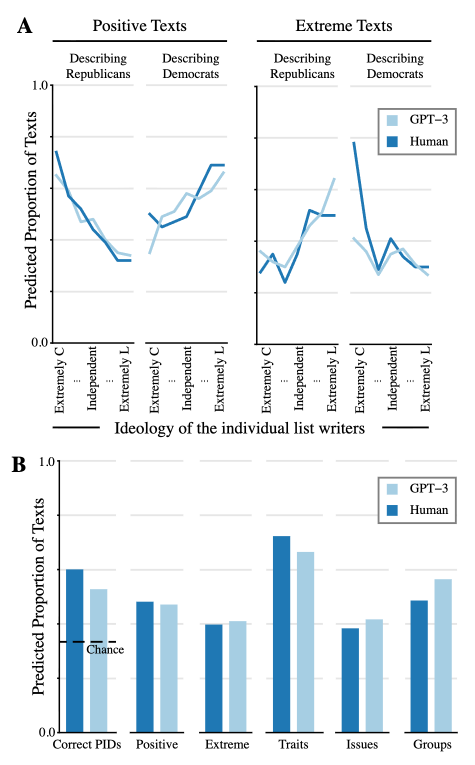
\includegraphics[width=0.9\linewidth]{../figures/gpt.lucid.png}
        \caption{Analysis of GPT-3 and human responses from the Lucid su; Fig 3 in \textcite{argyle2023out}}
      \end{figure}
  \end{columns}
\end{frame}


\begin{frame}
  \frametitle{AI as Subject: Pros and Cons}
  \begin{columns}[T,onlytextwidth]
    \column{0.7\textwidth}
      \footnotesize
      \begin{itemize}
      \item \textbf{Cons:}
      \begin{itemize}
        \item Poorly refelcting ``hard-to-reach \textcolor{red}{populations}'' \parencite{bollen2026nationally}; fail to capture experiential and cultural depth \parencite{pataranutaporn2025simulating}
        \item Reflect certain partisan \parencite{santurkar2023whose} or cultural \textcolor{red}{biases} \parencite{tao2024cultural}
        \item Closed to averages but less \textcolor{red}{variation} \parencite{bisbee2024synthetica}; have strong, varying biases and have low-variance in opinnion or attitudinal research\parencite{boelaert2025machine}; likely to both misportray and flatten demographic representations \parencite{wang2025large}; and tend to compress heterogeneity into
simplified typological structures \parencite{xie2025variance}
      \end{itemize}
    \end{itemize}
    \column{0.3\textwidth}
      \begin{figure}
        \centering
        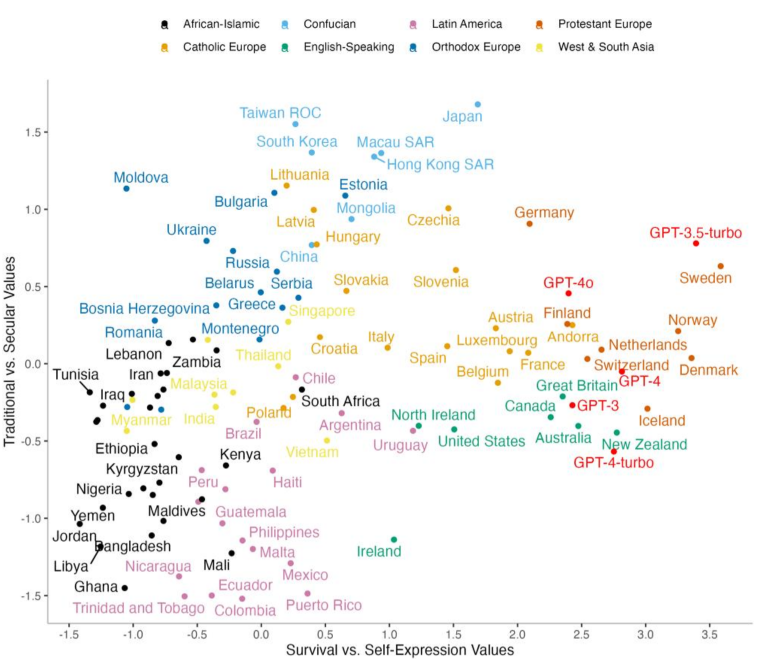
\includegraphics[width=\linewidth]{../figures/cultural.bias.png}
        \caption{Deviated LLM-generated answers related to values compared with different countries; Fig 1 in \textcite{tao2024cultural}}
      \end{figure}
  \end{columns}
\end{frame}


\begin{frame}
  \frametitle{AI as Subject: Pros and Cons}
  \begin{columns}[T,onlytextwidth]
    \column{0.7\textwidth}
      \footnotesize
      \begin{itemize}
      \item \textbf{Cons:}
      \begin{itemize}
        \item Poorly refelcting ``hard-to-reach \textcolor{red}{populations}'' \parencite{bollen2026nationally}; fail to capture experiential and cultural depth \parencite{pataranutaporn2025simulating}
        \item Reflect certain partisan \parencite{santurkar2023whose} or cultural \textcolor{red}{biases} \parencite{tao2024cultural}
        \item Closed to averages but less \textcolor{red}{variation} \parencite{bisbee2024synthetica}; have strong, varying biases and have low-variance in opinnion or attitudinal research\parencite{boelaert2025machine}; likely to both misportray and flatten demographic representations \parencite{wang2025large}; and tend to compress heterogeneity into
simplified typological structures \parencite{xie2025variance}
      \end{itemize}
    \end{itemize}
    \column{0.3\textwidth}
      \begin{figure}
        \centering
        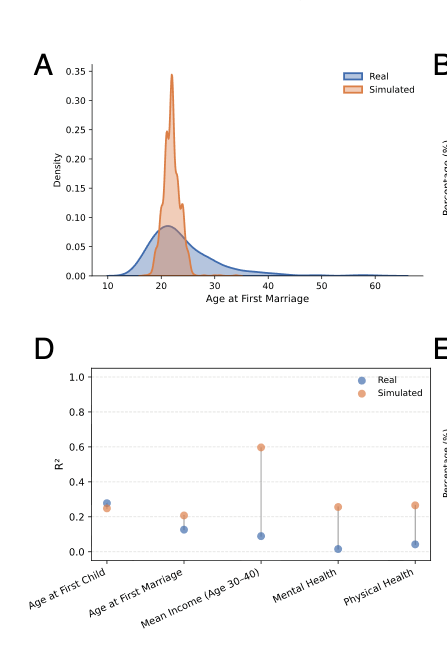
\includegraphics[width=\linewidth]{../figures/xie.eval.part.png}
        \caption{Failing to capture the dispersion of real-world distribution; Fig 3 in \textcite{xie2025variance}}
      \end{figure}
  \end{columns}
\end{frame}


\begin{frame}
  \frametitle{AI as Subject: Validation}
  \begin{columns}[T,onlytextwidth]
    \column{0.7\textwidth}
      \footnotesize
      \begin{itemize}
      \item \textbf{Cons:}
      \begin{itemize}
      \end{itemize}
    \end{itemize}
    \column{0.3\textwidth}
      \begin{figure}
        \centering
      \end{figure}
  \end{columns}
\end{frame}


\begin{frame}
  \frametitle{LLM as Method: Assistant}
  \begin{itemize}
    \item Writing, debugging, and translating analysis code
    \item Searching and summarizing literature
    \item Editing and polishing prose
    \item Data cleaning and wrangling
  \end{itemize}
  ~\\
  \textcolor{gray}{The researcher specifies the task; the LLM speeds up execution}
\end{frame}

\begin{frame}
  \frametitle{LLM as Method: Collaborator}
  \begin{itemize}
    \item Brainstorming research questions and hypotheses
    \item Critiquing research designs and identification strategies
    \item Proposing measures, robustness checks, and alternative explanations
    \item Agentic workflows: multi-step analysis with researcher oversight
  \end{itemize}
  ~\\
  \textcolor{gray}{The LLM contributes ideas; the researcher remains accountable}
\end{frame}

\begin{frame}
  \frametitle{LLM as Method: Evaluator}
  \begin{itemize}
    \item \textbf{Annotation}: zero- and few-shot text classification at scale
    \item \textbf{LLM-as-judge}: scoring quality, stance, or similarity
    \item \textbf{Review}: 
    \item \textbf{Replication}: To scale up reproducibility of empirical work \parencite{xu2026scaling} 
  \end{itemize}
\end{frame}

\begin{frame}
  \frametitle{LLM as Method: Choose the Right Tool}
      \small
      \begin{itemize}
        \item Consider a model as a function, $f(data, algo, object)$, the differences in each part would substantially shape their in-domain capabilities (like better coding or writing)
        \item In this sense, we may need to choose different models for different tasks, depending on their strengths and limitations
      \end{itemize}
\end{frame}

\begin{frame}
  \frametitle{LLM as Method: Choose the Right Tool}
  \begin{columns}[T,onlytextwidth]
    \column{0.48\textwidth}
      \small
      \begin{itemize}
        \item For example, you may expect \textcolor{blue}{Gemini Carbon} to excel in writing tasks whereas Claude Opus 5.5 outperforms in engineering
      \end{itemize}
    \column{0.5\textwidth}
      \begin{figure}
        \centering
        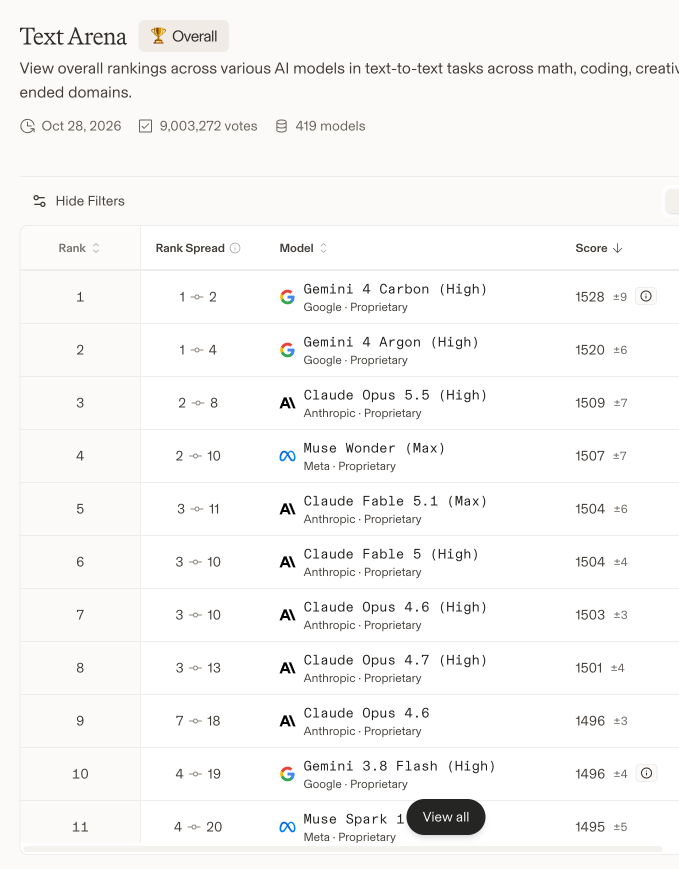
\includegraphics[width=0.8\linewidth]{bench.writing.png}
        \caption{Source: \url{https://arena.ai/leaderboard/chat/text} (Nov 3, 2026)}
      \end{figure}
  \end{columns}
\end{frame}
\begin{frame}
  \frametitle{LLM as Method: Choose the Right Tool}
  \begin{columns}[T,onlytextwidth]
    \column{0.48\textwidth}
      \small
      \begin{itemize}
        \item For example, you may expect Gemini Carbon to excel in writing tasks whereas \textcolor{orange}{Claude Opus 5.5} outperforms in engineering
        \item In general, model labs have different commercialization models, for business model optimized for engineering tasks may prioritize coding capabilities (e.g., Anthropic); please check benchmarks / review the literature / do a pilot test before using a model
      \end{itemize}
    \column{0.5\textwidth}
      \begin{figure}
        \centering
        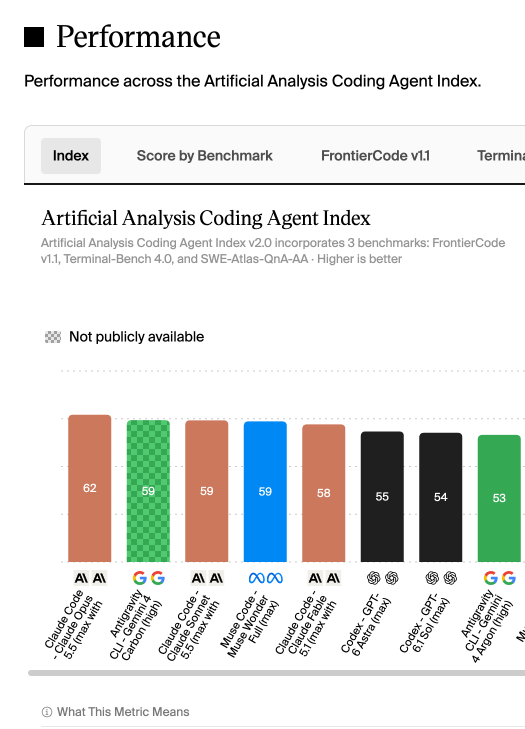
\includegraphics[width=0.8\linewidth]{bench.coding.png}
        \caption{Source: \url{https://artificialanalysis.ai/agents/coding-agents\#coding-agents-index} (Nov 3, 2026)}
      \end{figure}
  \end{columns}
\end{frame}

\begin{frame}
  \frametitle{LLM as Object}
  \begin{itemize}
    \item \textbf{Auditing models}: political slant, social bias, and value alignment
    \item \textbf{Effects on people}: persuasion, learning, labor, and well-being
    \item \textbf{Effects on information ecosystems}: AI-generated content and search
  \end{itemize}
\end{frame}

% =====================================================================
\sectionframe{Limitations}
% =====================================================================

\begin{frame}
  \frametitle{Limitations}
  \begin{enumerate}
    \item \textbf{Validity.} Outputs may not measure what we intend
    \item \textbf{Reproducibility.} Closed models, silent updates, and stochastic outputs
    \item \textbf{Bias.} Training data over-represent some groups and languages
    \item \textbf{Hallucination.} Fabricated facts and citations
    \item \textbf{Ethics.} Privacy, consent, and data sent to third parties
    \item \textbf{Over-reliance.} Deskilling and unexamined defaults
  \end{enumerate}
\end{frame}

% % =====================================================================
% \sectionframe{Forward-looking}
% % =====================================================================

% \begin{frame}
%   \frametitle{Recent Advances}
%   \begin{itemize}
%     \item \textbf{Model transparency}: prefer open-weight models and document versions
%   \end{itemize}
%   ~\\
%   \textcolor{gray}{From AI as a tool to AI as a research partner---with guardrails}
% \end{frame}

% =====================================================================
\sectionframe{Takeaways}
% =====================================================================

\begin{frame}
  \frametitle{Takeaways}
  \begin{itemize}
    \item AI models (which includes LLMs) can be subjects, objects, and \textcolor{blue}{methods} in quantitative social research
    \item \textcolor{blue}{As methods}, they are expected to be used in a responsible way in which validity, reproducibility, bias, hallucination, ethics, and over-reliance are carefully considered
    \item \textcolor{blue}{Like any other methods}, they evolve in a quick (and potentially quicker pace), but our tastes of good questions remain relatively central to research (and industrial jobs)
    \item ``... Be skeptic... don't panic!'' \parencite{angrist2009mostly}
  \end{itemize}
\end{frame}


\begin{frame}
  \frametitle{Takeaways}
  \begin{itemize}
    \item ``... Be skeptic... don't panic!'' \parencite{angrist2009mostly}
  \end{itemize}
  \begin{figure}
    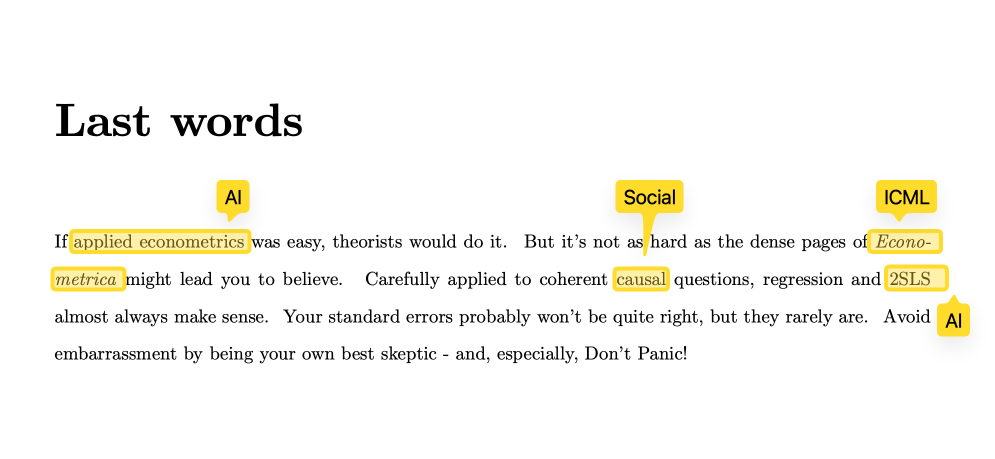
\includegraphics[width=1\textwidth]{../figures/dont.panic.png}
    \caption{Source: \textcite{angrist2009mostly}}
  \end{figure}
\end{frame}

% =====================================================================
\sectionframe{Resources}
% =====================================================================

\begin{frame}
  \frametitle{Resources}
  \begin{itemize}
      \item Locate the most appropriate AI model for your task
        \begin{itemize}
          \item Artificial analysis \url{https://artificialanalysis.ai/}
          \item Arena.ai, blind benchmarking for AI models \url{https://arena.ai/leaderboard/}
        \end{itemize}
      \item Find problems in your manuscript
        \begin{itemize}
          \item Refine, publication-level technical review; adopted by AEA \url{https://www.refine.ink/}
          \item OpenAIReview, opensource solution of multi-agent manuscript review by UChicago HAI \url{https://github.com/ChicagoHAI/OpenAIReview}
          \end{itemize}
      \item Doublecheck references and citations
        \begin{itemize}
          \item CiteVerify, ``a local tool for verifying references in research papers'', \url{https://github.com/cuihuash/CiteVerify}
          \end{itemize}
      \item Manage multiple AI models and services
        \begin{itemize}
          \item For macOS, magpie, local AI router management for mac \url{https://github.com/yetone/magpie} 
          \item For other platforms, cc-switch, \url{https://github.com/farion1231/cc-switch}
        \end{itemize}
      \item Read scientific literature using your own language
        \begin{itemize}
          \item PDFMathReader, read scientific PDFs in your language \url{https://github.com/PDFMathTranslate/PDFMathReader}
        \end{itemize}
  \end{itemize}
\end{frame}



% {
%   \setbeamercolor{background canvas}{bg=black}
%   \begin{frame}
%     \begin{center}
%       \Huge{\textcolor{white}{Acknowledgments}}
%     \end{center}
%     \vspace{1cm}
%     \normalsize{\textcolor{white}{We thank \ldots. All errors are our own.}}
%   \end{frame}
% }

\sectionframe{References}

\begin{frame}[allowframebreaks]
  \frametitle{References}
  \begingroup
  \referencesize\color{black}
  \printbibliography[notkeyword=chinese,heading=none]
  \endgroup
\end{frame}


\end{document}
